\documentclass[conference]{IEEEtran}
\IEEEoverridecommandlockouts
\usepackage{cite}
\usepackage{amsmath,amssymb,amsfonts}
\usepackage{algorithmic}
\usepackage{graphicx}
\usepackage{textcomp}
\usepackage{xcolor}
\usepackage{booktabs}
\usepackage{stfloats}

\def\BibTeX{{\rm B\kern-.05em{\sc i\kern-.025em b}\kern-.08em
    T\kern-.1667em\lower.7ex\hbox{E}\kern-.125emX}}

\begin{document}

\title{Subject-Vector Model Merging for Motor Imagery EEG Foundation Models}

\author{
\IEEEauthorblockN{Anonymous Authors}
\IEEEauthorblockA{Draft manuscript for discussion}
}

\maketitle

\begin{abstract}
Recent EEG foundation models have shown promising capability in learning generalizable representations from large-scale unlabeled EEG recordings. However, substantial inter-subject variability still limits their direct deployment to downstream EEG tasks, where subject-specific adaptation is often required for reliable performance. This practice produces one adapted model per subject, leading to rapidly increasing storage and deployment costs in large-subject scenarios. To address this limitation, we investigate training-free post-hoc merging of subject-adapted EEG foundation models. Given multiple subject-specific models adapted from the same pretrained EEG foundation model, the goal is to obtain a single unified model while preserving subject-level performance. We propose a subject-wise weighted model merging strategy, which assigns different merging weights to different subject-adapted models to reduce weight-space conflicts induced by inter-subject distribution shifts. Experiments on two motor imagery EEG benchmarks, BNCI2014004 and BNCI2015001, show that the proposed method achieves average accuracies of 80.52\% and 75.00\%, outperforming standard weight averaging by 1.88\% and 2.02\%, respectively. Compared with the average cross-subject transfer performance of individual subject-adapted models, the proposed merged model further improves accuracy by 6.60\% and 10.90\% on the two datasets. Although fully individualized subject-specific models remain a strong empirical upper-bound solution, the proposed method substantially narrows the performance gap while requiring only one deployed model. These results demonstrate that training-free post-hoc model merging is a promising strategy for scalable and storage-efficient deployment of EEG foundation models.
\end{abstract}

\begin{IEEEkeywords}
EEG foundation model, subject vector, model merging, motor imagery, subject adaptation
\end{IEEEkeywords}

\section{Introduction}
Large-scale self-supervised pretraining has become an important direction for EEG representation learning. Representative EEG foundation models, including BENDR~\cite{b1}, LaBraM~\cite{b2}, and CBraMod~\cite{b3}, show that generic neural representations can be learned from large collections of EEG recordings and transferred to downstream brain-computer interface tasks. This is particularly appealing for motor imagery (MI) decoding, where labeled data are limited and expensive to collect. However, despite the promise of pretrained EEG representations, MI decoding remains strongly affected by inter-subject variability, and direct zero-shot deployment is often insufficient.

A common practical solution is to adapt the same pretrained model separately to each subject. This subject-specific adaptation often improves performance, but it also creates a set of isolated subject-adapted endpoints. More importantly, the issue is not only that multiple checkpoints are produced, but that adaptation knowledge becomes fragmented across them. Each subject-specific model captures some useful knowledge about how the pretrained representation should be adjusted for MI decoding, yet this knowledge remains distributed across separate model endpoints rather than consolidated into a unified population-level model.

This motivates the following question: can multiple subject-adapted endpoints be merged into a single population-level model without revisiting pooled raw EEG data? In other words, given several subject-specific models derived from the same pretrained EEG foundation model, can we fuse their adaptation knowledge post hoc and obtain a shared model that remains broadly useful across subjects? This problem differs from conventional signal-level, feature-level, or decision-level fusion, because the object to be fused is not EEG data or predictions, but the adapted model parameters themselves.

Let $\theta_0$ denote the pretrained EEG foundation model and let $\theta_s$ denote the model adapted to subject $s$. We define the corresponding parameter displacement as
\begin{equation}
v_s = \theta_s - \theta_0.
\end{equation}
We refer to $v_s$ as a \emph{subject vector}. This terminology is intentional. In conventional task arithmetic, parameter offsets are typically associated with different tasks. In our setting, however, all models solve the same MI decoding task; what differs is the subject to which the model has been adapted. Therefore, the relevant variation is better described at the subject level rather than the task level.

At the same time, subject-vector merging is not a trivial extension of standard task-vector averaging. A subject vector may contain multiple components: a shared task-related adaptation component that is beneficial across subjects, a subject-specific component that reflects individual neural or recording characteristics, and a noise or overfitting component that may not transfer well. Uniform averaging implicitly assumes that all subject vectors contribute equivalently, while global scaling only adjusts the overall update magnitude. Neither assumption fully addresses the more fundamental issue that different subject vectors may have different degrees of compatibility. Thus, the key challenge is not merely how strongly to merge subject-adapted models, but how their heterogeneous components should be composed.

In this work, we study this problem in a controlled setting using MIRepNet as the common pretrained backbone. The goal is not to benchmark multiple architectures, but to isolate and analyze subject-level mergeability in motor imagery EEG foundation models under a fixed backbone. Within this setting, we formulate post-hoc fusion as a subject-vector merging problem and compare uniform, globally scaled, and subject-scaled merging strategies. Experiments on BNCI2014004 and BNCI2015001 show that a single merged model can recover a substantial portion of the benefit of subject-specific adaptation, while also revealing that subject vectors contain both shared and non-shared components.

\begin{table*}[!t]
\caption{Main results on the two motor imagery datasets. Values are reported as average accuracy $\pm$ standard deviation (\%). The top row is the personalized oracle upper bound, and the lower block compares single shared-model baselines.}
\label{tab:main_results}
\centering
\scriptsize
\setlength{\tabcolsep}{5pt}
\renewcommand{\arraystretch}{1.05}
\begin{tabular}{p{4.2cm}ccp{4.1cm}}
\toprule
Method & BNCI2014004 Acc. $\pm$ Std. & BNCI2015001 Acc. $\pm$ Std. & Role \\
\midrule
Subject-specific FT on own subject & \textbf{82.31 $\pm$ 12.66} & \textbf{81.13 $\pm$ 13.49} & personalized oracle upper bound \\
Pooled joint training & 77.94 $\pm$ 12.85 & 73.63 $\pm$ 11.96 & raw-data joint training baseline \\
\specialrule{1.1pt}{0pt}{0pt}
Weight Avg & 78.64 $\pm$ 10.52 & 72.98 $\pm$ 13.62 & standard post-hoc fusion \\
Best global-scaled TA & 80.22 $\pm$ 9.36 & 73.04 $\pm$ 13.57 & best global strength only \\
Oracle subject-scaled TA (proposed) & \textbf{80.52 $\pm$ 10.48} & \textbf{75.00 $\pm$ 13.15} & proposed subject-wise composition \\
\bottomrule
\end{tabular}
\end{table*}

\section{Related Work}
\subsection{EEG Foundation Models}
EEG foundation models seek to learn reusable neural representations from large-scale unlabeled or weakly labeled recordings. BENDR~\cite{b1} demonstrated early that self-supervised pretraining with Transformer-based sequence modeling can improve EEG transfer learning. More recent models such as LaBraM~\cite{b2} and CBraMod~\cite{b3} further scale data volume, model size, and architectural inductive bias, leading to stronger general-purpose EEG features. However, the downstream use of these models still commonly relies on subject-specific fine-tuning, especially in motor imagery tasks where inter-subject variability remains substantial.

\subsection{Model Merging}
Post-hoc parameter merging has recently emerged as a lightweight alternative to joint retraining. Model soups~\cite{b4} show that averaging fine-tuned models can improve generalization without increasing inference cost. Task arithmetic~\cite{b5} interprets fine-tuning updates as task vectors that can be combined in weight space. More generally, work on permutation symmetries and low-loss connectivity~\cite{b6,b7} provides geometric intuition for why separately adapted models can sometimes be merged successfully. Our work is inspired by this line of research, but differs in both setting and objective: rather than merging generic task-specialized models, we merge subject-adapted EEG foundation models and focus on preserving performance across multiple subjects with a single deployment checkpoint.

\section{Method}
\subsection{Problem Formulation}
Let $\theta_{0}$ denote a pretrained EEG foundation model and let $\theta_{s}$ denote the model obtained after adapting $\theta_{0}$ to subject $s$, where $s \in \{1,\ldots,S\}$. The objective is to construct a single merged model $\theta_{\mathrm{merge}}$ from $\{\theta_{s}\}_{s=1}^{S}$ such that the merged model remains broadly useful across subjects while avoiding the need to deploy $S$ separate adapted checkpoints.

For convenience, we define the subject-specific adaptation vector
\begin{equation}
\Delta_{s} = \theta_{s} - \theta_{0}.
\end{equation}
Each $\Delta_s$ captures how subject $s$ modifies the pretrained model.

\subsection{Baseline Merging Strategies}
The no-adaptation reference uses the pretrained EEG foundation model directly, which in our notation is equivalent to setting the global scaling factor to zero:
\begin{equation}
\theta_{\beta=0} = \theta_{0}.
\end{equation}
This baseline indicates how much performance can be obtained without injecting any downstream task vector.

Because all subject-adapted models share the same pretrained initialization, direct equal-weight parameter averaging is identical to uniform task arithmetic:
\begin{equation}
\theta_{\mathrm{uni}} = \frac{1}{S}\sum_{s=1}^{S}\theta_{s}
= \theta_{0} + \frac{1}{S}\sum_{s=1}^{S}\Delta_{s}.
\end{equation}
This baseline corresponds to uniform TA / weight averaging with $\beta=1$ and assumes that all subject updates should contribute equally.

A stronger global-only baseline keeps the uniform subject weights but rescales the shared task vector with a single scalar:
\begin{equation}
\theta_{\mathrm{global}}(\beta) = \theta_{0} + \beta\frac{1}{S}\sum_{s=1}^{S}\Delta_{s}.
\end{equation}
When $\beta=1$, $\theta_{\mathrm{global}}(\beta)$ reduces to uniform TA / weight averaging; tuning $\beta$ yields the best global-scaled TA baseline.

\setcounter{figure}{1}
\begin{figure*}[!t]
\centering
\makebox[\textwidth][c]{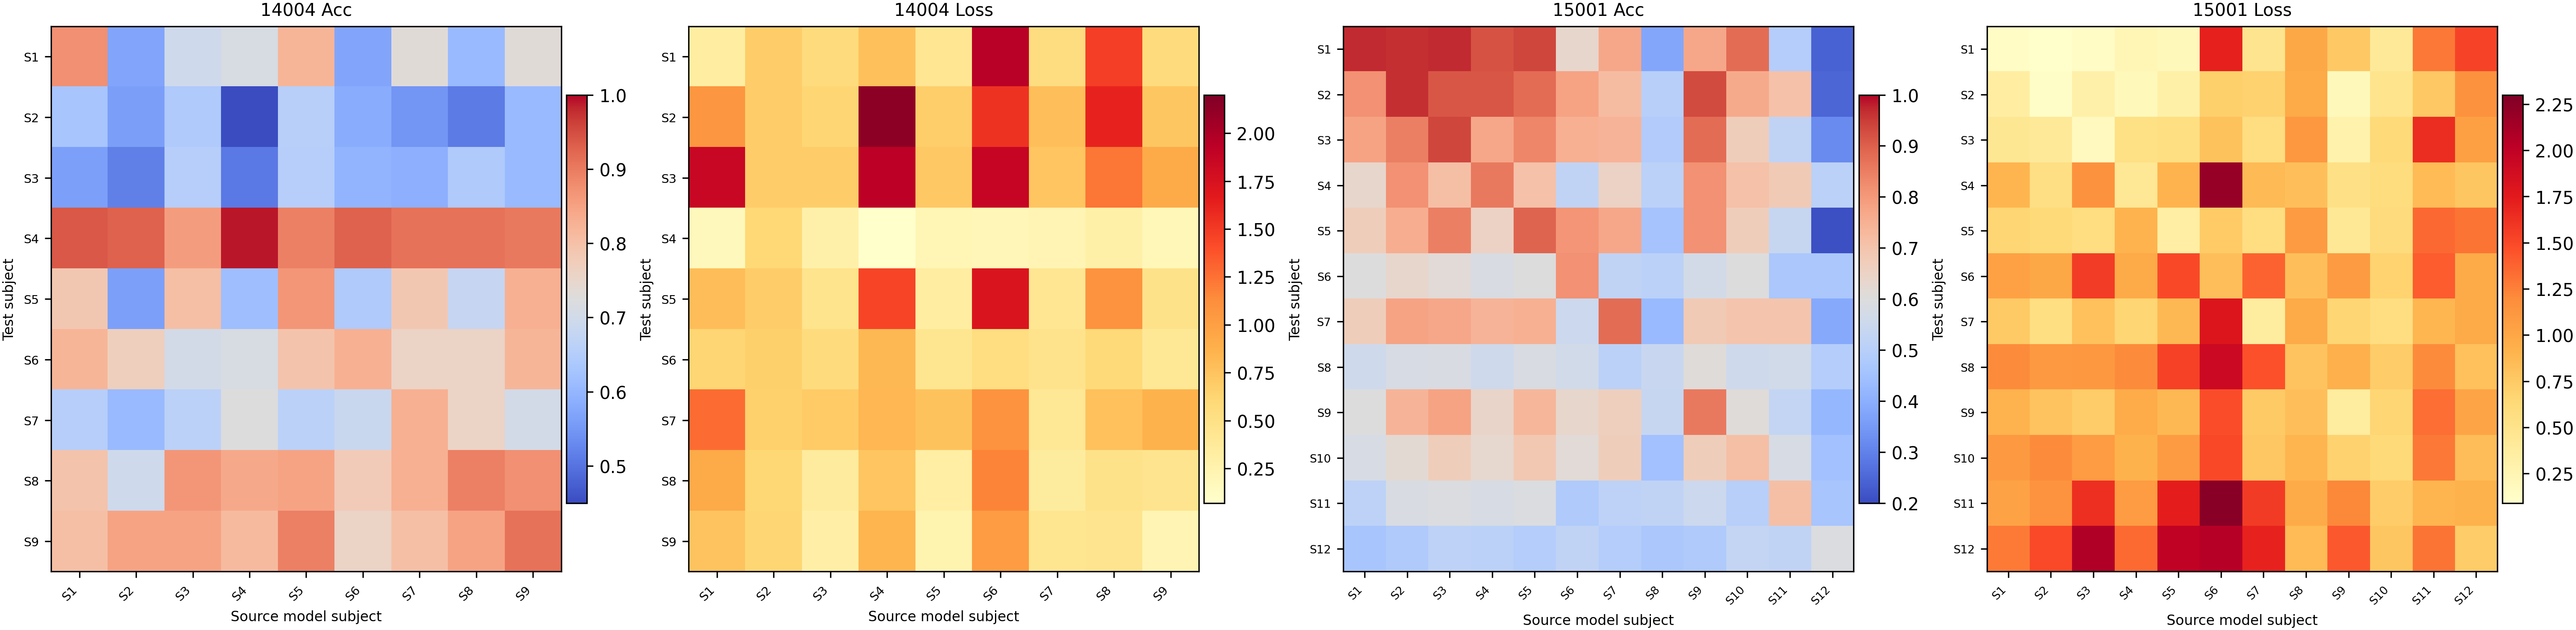
\includegraphics[width=1.08\textwidth]{figures/cross_subject_compatibility.png}}
\caption{Cross-subject endpoint compatibility on BNCI2014004 and BNCI2015001. Rows denote test subjects and columns denote source subject-specific models. Higher off-diagonal accuracy and lower off-diagonal loss indicate stronger cross-subject endpoint compatibility and, in turn, easier post-hoc mergeability.}
\label{fig:compatibility}
\end{figure*}
\setcounter{figure}{0}

\subsection{Subject-Wise Weighted Merging}
Our method retains the same task-vector perspective but uses a two-stage weighting scheme. We first assign each adapted model a raw subject score $\alpha_s$ and normalize these scores into subject weights:
\begin{equation}
w_s = \frac{\alpha_s}{\sum_{k=1}^{S}\alpha_k}.
\end{equation}
The normalized weights $w_s$ determine the relative contribution of each subject and satisfy $\sum_{s=1}^{S}w_s = 1$. The final merged model is then computed as
\begin{equation}
\theta_{\mathrm{swm}} = \theta_{0} + \beta\sum_{s=1}^{S}w_s(\theta_s-\theta_0),
\label{eq:swm}
\end{equation}
where $\beta$ controls the overall magnitude of the merged update. Equivalently, \eqref{eq:swm} can be written as $\theta_{\mathrm{swm}} = \theta_0 + \beta\sum_{s=1}^{S}w_s\Delta_s$. When all $\alpha_s$ are equal and $\beta=1$, \eqref{eq:swm} reduces to uniform task-vector averaging. In this work, we use one scalar score per subject, which keeps the merged model compact and easy to interpret.

The intuition is straightforward. Subject-adapted models do not contribute equally to a common deployment model because their updates reflect different subject-specific distributions. Some adaptations are more compatible with the shared parameter basin, while others may introduce stronger interference when averaged indiscriminately. The normalized weights $w_s$ therefore provide a lightweight mechanism to suppress conflicting updates and emphasize subject models that better align with the overall merged solution, while $\beta$ adjusts how strongly the combined subject adaptation is injected into the base model.

\subsection{Practical Properties}
The proposed method is training-free at merge time. Once subject-adapted models, the raw subject scores $\alpha_s$, and the global scaling factor $\beta$ are specified, the final checkpoint is obtained by a single pass over parameters, with no further backpropagation. This property is attractive for deployment because only one merged model needs to be stored online. In contrast, fully individualized deployment requires retaining all subject-specific models. The current formulation also remains flexible: more fine-grained weighting schemes, such as layer-wise or block-wise weights, can be incorporated in future work without changing the basic framework.

\section{Experimental Setup}
\subsection{Datasets}
We evaluate on two public motor imagery EEG benchmarks. BNCI2014004 corresponds to BCI Competition IV Dataset 2b~\cite{b8} and contains data from nine subjects performing binary motor imagery classification. BNCI2015001 contains data from twelve subjects and is a widely used benchmark for cross-subject motor imagery analysis~\cite{b9}. These two datasets provide complementary testbeds for studying subject variability and multi-subject deployment.

\subsection{Evaluation Protocols}
All subject-specific models are adapted from the same pretrained EEG foundation model, after which they are merged or evaluated using the following protocols.

\textbf{Pretrained / no task vector ($\beta=0$):} the pretrained EEG foundation model $\theta_0$ is evaluated directly without downstream adaptation.

\textbf{Single-subject models on all subjects:} each subject-specific fine-tuned model is evaluated on all subjects, and the resulting accuracies are averaged. This quantifies cross-subject single-source transfer.

\textbf{Subject-specific FT on own subject (oracle):} each fine-tuned model is evaluated only on its corresponding subject. We treat this setting as an empirical personalized upper bound.

\textbf{Pooled joint training:} a single downstream model is trained on pooled multi-subject data and then evaluated on all subjects.

\textbf{Uniform TA / weight average ($\beta=1$):} the subject task vectors are merged uniformly, which is equivalent to direct equal-weight parameter averaging under the shared initialization.

\textbf{Best global-scaled TA:} the subject task vectors are still merged uniformly, but a dataset-specific global scaling factor $\beta$ is selected to maximize performance.

\textbf{Oracle subject-scaled TA (proposed):} a single merged model is constructed using \eqref{eq:swm} with dataset-specific raw subject scores $\alpha_s$ and a global scaling factor $\beta$.

We report average classification accuracy and standard deviation. The main comparison focuses on the deployment trade-off between the personalized oracle, pooled joint training, and training-free task-arithmetic variants.

\section{Results and Discussion}
\subsection{Main Results}
Table~\ref{tab:main_results} summarizes the main deployment comparison. The personalized oracle remains the strongest overall setting, but among single shared-model solutions the proposed oracle subject-scaled TA achieves the best performance on both datasets. On BNCI2014004, it reaches $80.52\%$, outperforming pooled joint training, uniform TA / weight averaging, and best global-scaled TA by $2.58$, $1.88$, and $0.30$ percentage points, respectively. On BNCI2015001, it reaches $75.00\%$, outperforming the same three baselines by $1.37$, $2.02$, and $1.96$ percentage points.

For completeness, the pretrained / no-task-vector reference achieves $38.76\% \pm 13.64\%$ on BNCI2014004 and $41.96\% \pm 13.62\%$ on BNCI2015001, while the average cross-subject transfer of single-subject models reaches $73.92\% \pm 3.47\%$ and $64.10\% \pm 10.06\%$, respectively.

These results support two observations. First, subject-adapted models remain much stronger on their own subjects than in cross-subject transfer, which confirms that subject variability is a central bottleneck. Second, scaling the shared task vector with a single global factor yields limited benefit, whereas subject-specific scaling produces a more reliable shared deployment model.

\begin{figure}[!t]
\centering
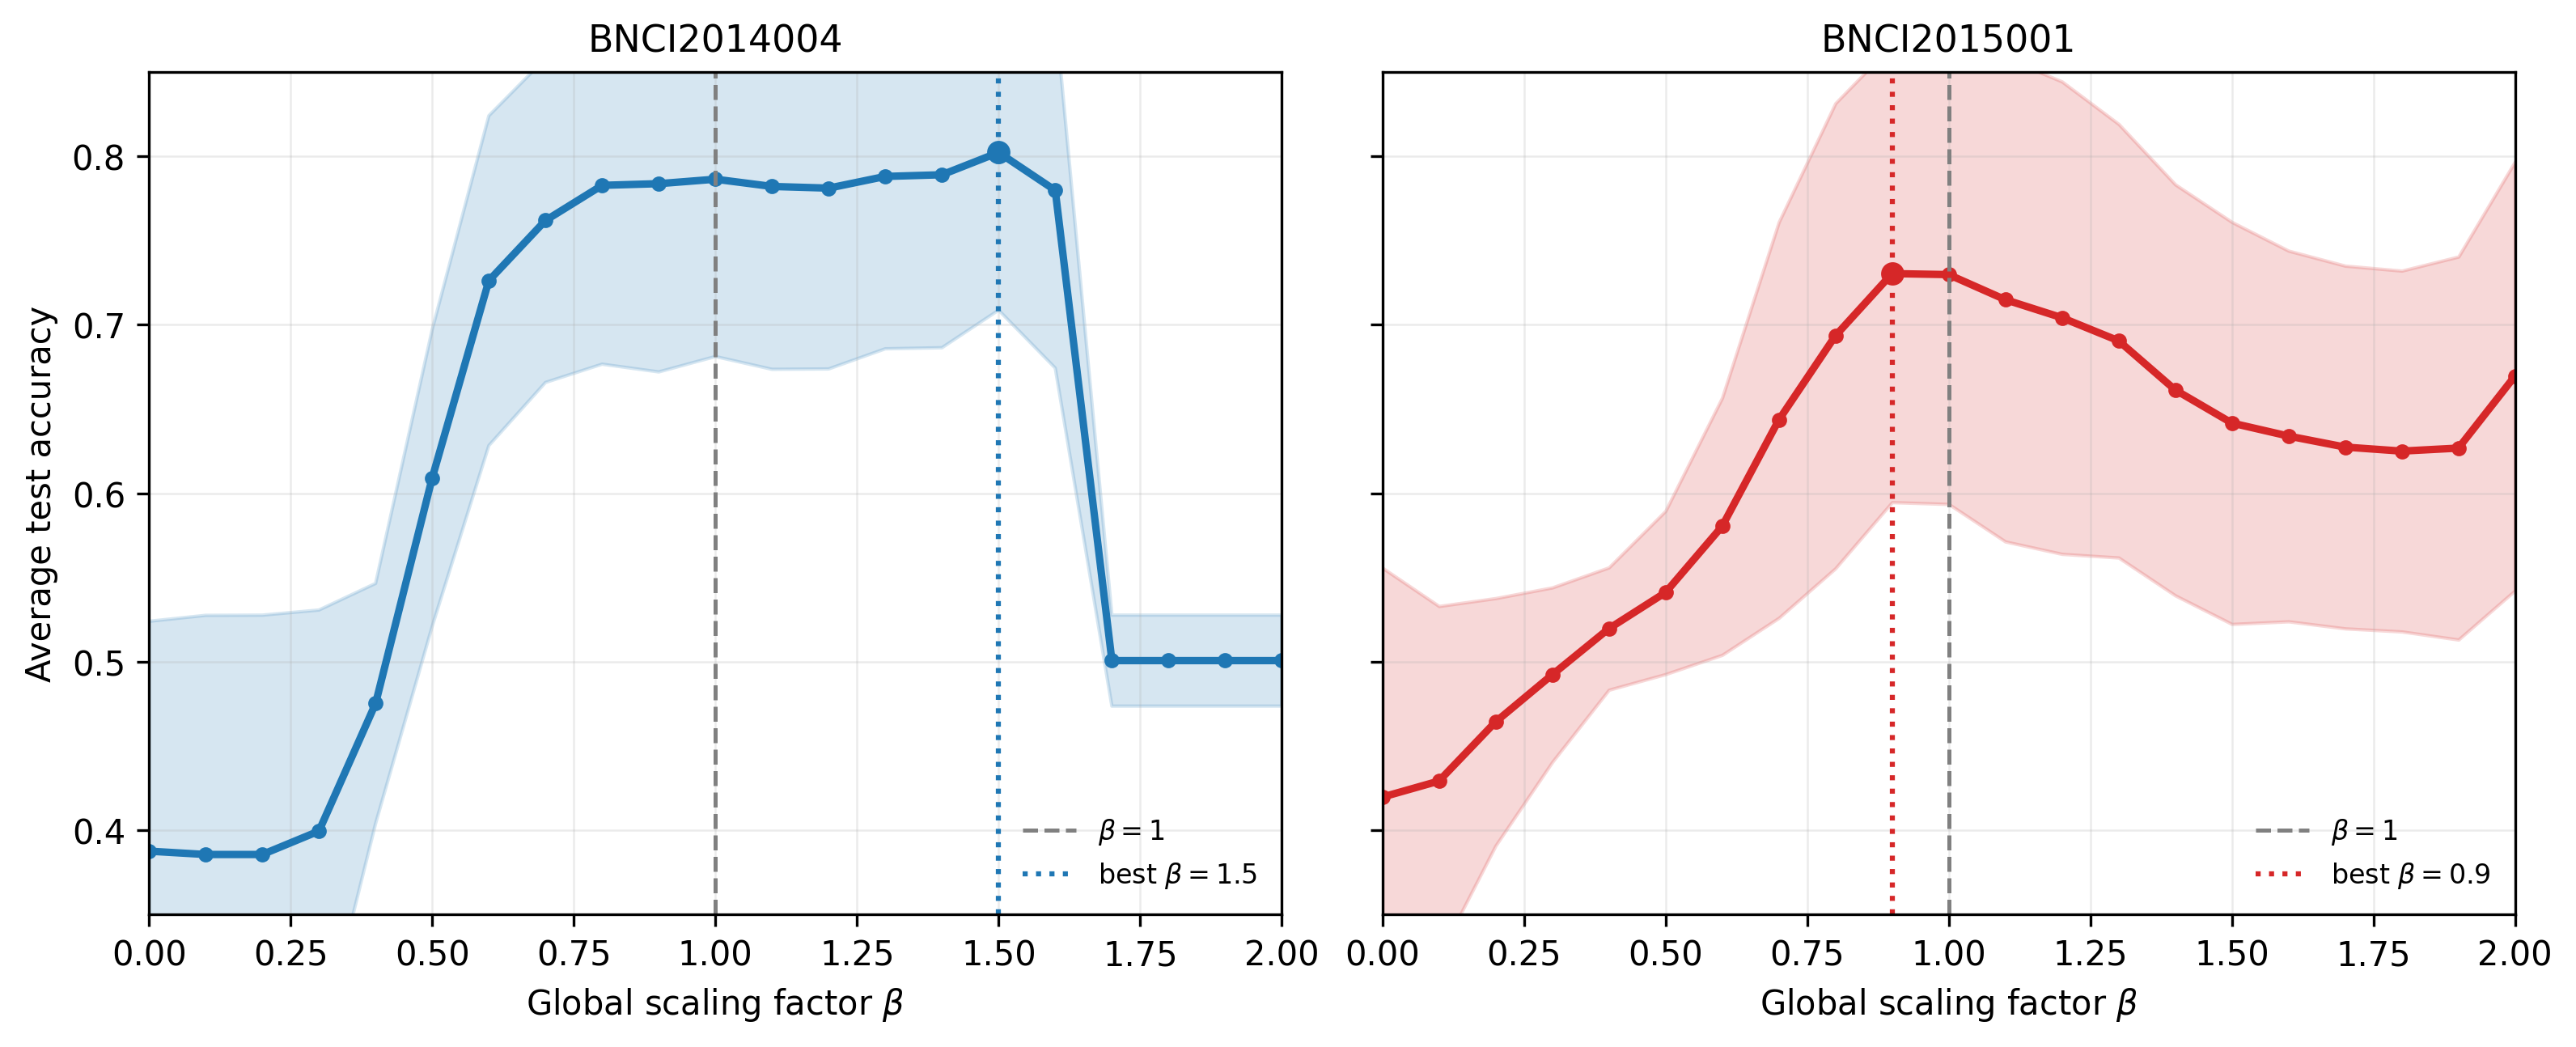
\includegraphics[width=0.98\columnwidth]{figures/beta_sweep_curves.png}
\caption{Average test accuracy under global task-vector scaling on the two datasets. Shaded bands indicate one standard deviation across subjects. Both datasets benefit from moving away from $\beta=0$, but the shape of the sweep differs markedly across datasets.}
\label{fig:beta_sweep}
\end{figure}

\subsection{Discussion}
\textbf{Overall finding.} Table~\ref{tab:main_results} shows that EEG foundation models still require subject-specific adaptation for competitive motor imagery decoding. The pretrained no-task-vector baseline is only $38.76\%$ on BNCI2014004 and $41.96\%$ on BNCI2015001, whereas own-subject fine-tuning reaches $82.31\%$ and $81.13\%$, respectively. Uniform TA / weight averaging already recovers a substantial portion of this gap, reaching $78.64\%$ and $72.98\%$, and the proposed oracle subject-scaled merge further improves these numbers to $80.52\%$ and $75.00\%$. The remaining gap to the own-subject oracle is small on BNCI2014004 ($1.79$ points) but larger on BNCI2015001 ($6.13$ points), which already suggests that subject vectors are useful but not uniformly mergeable.

\textbf{Difference from pooled joint training.} The comparison to pooled joint training highlights the distinctive nature of model fusion for EEG foundation models. Pooled joint training reaches $77.94\%$ on BNCI2014004 and $73.63\%$ on BNCI2015001, while oracle subject-scaled TA improves on these results by $2.58$ and $1.37$ percentage points, respectively. Even uniform TA is competitive with pooled training: it is slightly better on BNCI2014004 and only slightly worse on BNCI2015001. This pattern suggests that multi-subject adaptation is not purely a matter of exposing the model to more pooled data. Because subject heterogeneity is substantial in EEG, the pooled training objective can contain gradient conflict across subjects, so joint optimization does not necessarily dominate post-hoc fusion in a stable way.

\textbf{Global scaling analysis.} The $\beta$ sweep in Fig.~\ref{fig:beta_sweep} shows that the averaged task vector already contains a shared motor imagery adaptation direction. On BNCI2014004, the average accuracy rises from $38.76\%$ at $\beta=0$ to a peak of $80.22\%$ at $\beta=1.5$, and the curve remains near its optimum over a relatively broad range from about $\beta=0.8$ to $\beta=1.5$. On BNCI2015001, the same procedure rises from $41.96\%$ to a peak of $73.04\%$ at $\beta=0.9$, but the near-optimal region is much narrower and performance decays more steadily beyond $\beta\approx 1.0$. This indicates that both datasets share a useful averaged adaptation direction, but BNCI2014004 is more tolerant to movement along that direction, whereas BNCI2015001 occupies a narrower and more fragile region in weight space.

\textbf{Cross-subject endpoint compatibility.} Fig.~\ref{fig:compatibility} explains why the two datasets respond differently to merging. On BNCI2014004, the mean diagonal accuracy is $82.31\%$, but the mean off-diagonal accuracy remains relatively high at $72.87\%$, with a corresponding off-diagonal loss of $0.783$. On BNCI2015001, the mean diagonal accuracy is similar at $81.13\%$, yet the mean off-diagonal accuracy drops to $62.55\%$ and the off-diagonal loss increases to $0.973$. Equivalently, the diagonal-to-off-diagonal accuracy gap is only $9.44$ points on BNCI2014004 but $18.58$ points on BNCI2015001. The BNCI2014004 matrix still contains hard cases, but its off-diagonal transfer remains comparatively dense and low-loss, with subjects such as S4 transferring well across many endpoints. In contrast, BNCI2015001 exhibits a clearer hard-subject tail: test subjects such as S12, S11, S8, and S6 have markedly lower off-diagonal transfer and consistently higher loss. This suggests that dataset-dependent mergeability is driven by endpoint compatibility rather than by overall task difficulty alone.

\textbf{Subject-scaled oracle interpretation.} Best global-scaled TA still underperforms the subject-scaled oracle by $0.30$ points on BNCI2014004 and by $1.96$ points on BNCI2015001. Because the global baseline already chooses the best scalar $\beta$, this residual gap cannot be explained by overall update strength alone. Instead, it points to a direction-composition problem: different subject vectors likely contain a mixture of shared adaptation components, redundant directions, hard-subject compensation directions, and non-mergeable subject-specific updates. Subject-wise scaling is therefore informative not only because it improves accuracy, but also because it reveals that the main remaining obstacle is how subject directions are composed, rather than how strongly the final merged update is scaled.

\textbf{Limitations and future work.} The current formulation is best viewed as an oracle diagnostic rather than a deployable selection rule. It assumes access to subject-level signals strong enough to choose the raw subject scores $\alpha_s$ and the global scaling factor $\beta$ after adaptation. A key next step is to estimate subject compatibility without labeled validation data, for example through checkpoint similarity, batch-normalization or feature-statistic proxies, Fisher-style importance surrogates, predictive confidence statistics, or other data-free measures of endpoint alignment. Turning the present oracle into a validation-free merge policy is therefore a central direction for future work.

\section{Conclusion}
This paper studies training-free post-hoc merging of subject-adapted EEG foundation models for scalable multi-subject deployment. We formulate the problem at the parameter level and propose a subject-wise weighted merging strategy that modulates how much each subject adaptation contributes to the final unified model. Experiments on BNCI2014004 and BNCI2015001 show that the proposed method consistently outperforms standard averaging baselines and substantially reduces the gap to fully individualized deployment while requiring only one deployed checkpoint. These results suggest that model merging is a promising direction for storage-efficient and scalable EEG foundation model deployment.

\bibliographystyle{IEEEtran}
\bibliography{reference}

\end{document}
